\documentclass[11pt,a4paper]{article}
\usepackage[utf8]{inputenc}
\usepackage[T1]{fontenc}
\usepackage[spanish]{babel}
\usepackage[margin=2.5cm]{geometry}
\usepackage{graphicx,booktabs,csquotes,float,tabularx}
\usepackage[backend=biber,style=ieee,sorting=none]{biblatex}
\addbibresource{referencias.bib}
\DefineBibliographyStrings{spanish}{artno={art\adddot}}
\usepackage{xurl}
\usepackage[hidelinks]{hyperref}

\begin{document}
\begin{titlepage}
  \centering
  {\Large Universidad Técnica Estatal de Quevedo\par}
  Facultad de ciencias de la computacion
  Ingeniería de Software\par
  Aplicaciones Distribuidas (ISR-701)\par
  \vfill
  {\Large TA-IND-01\par}
  {\LARGE Análisis crítico comparativo de un sistema distribuido\par}
  % Agregar el sistema una vez confirmada la elección en el foro.
  \vfill
  Melanie Michelle Muñoz Vera\par
  % Confirmar el paralelo y la fecha de entrega.
  \url{https://github.com/Melanir/isr701-ta-ind-01}\par
  \vfill
  Borrador de estructura
\end{titlepage}

\section*{Resumen}
Este informe analiza Apache Cassandra como sistema distribuido y lo compara con MongoDB para identificar cómo sus decisiones de replicación afectan la disponibilidad y la consistencia. Se configuraron tres nodos de Cassandra en Docker, en una sola computadora, con factor de replicación tres. Se insertó una fila con el nivel \texttt{ALL} y se consultó antes, durante y después de detener dos contenedores. Con todos los nodos activos, \texttt{ONE} y \texttt{QUORUM} devolvieron la fila. Durante la caída, \texttt{ONE} siguió respondiendo y \texttt{QUORUM} falló porque exigía dos réplicas accesibles. Tras recuperar los nodos, \texttt{QUORUM} volvió a funcionar. La comparación documental muestra que MongoDB utiliza una mayoría de votantes para mantener o elegir un primario, mientras Cassandra exige un número de respuestas según el nivel de cada operación. Los resultados respaldan la elección de \texttt{ONE} para lecturas que toleran datos desactualizados. La prueba mide si la consulta puede completarse. Evaluar la latencia, las escrituras concurrentes y las particiones de red requeriría experimentos adicionales.

\section{Introducción}
Apache Cassandra es una base de datos NoSQL de columnas anchas. La usan equipos que necesitan distribuir grandes volúmenes de datos entre varios servidores y mantener el servicio disponible cuando falla un nodo. Un ejemplo es Discord. Su equipo de ingeniería documentó que, a principios de 2022, almacenaba billones de mensajes en un clúster de 177 nodos Cassandra. El crecimiento también trajo problemas de latencia y mantenimiento que motivaron su migración posterior a ScyllaDB \cite{cassandra5dynamo,ingram2023discord}.

Este informe analiza cómo el nivel de consistencia afecta la posibilidad de leer un dato cuando se pierden réplicas. La prueba utiliza tres nodos Cassandra en Docker y compara la misma lectura con \texttt{ONE} y \texttt{QUORUM} antes, durante y después de detener dos nodos. Como contexto, se toman estudios que comparan configuraciones de consistencia de Cassandra, MongoDB y Redis en la nube \cite{ferreira2025ycsb,ferreira2024cloud}. La comparación arquitectónica con MongoDB se apoya en su documentación sobre conjuntos de réplicas \cite{mongodb8replication}. La práctica local se limita a Cassandra y observa si la consulta puede completarse.

\section{Arquitectura de Cassandra}
Cassandra funciona como un clúster de nodos pares. El nodo que recibe una solicitud del cliente actúa como coordinador de esa operación y se comunica con las réplicas que corresponden al dato. Los nodos mantienen información sobre la membresía y el estado del clúster mediante el protocolo \textit{gossip} \cite{cassandra5dynamo}.

Para ubicar los datos, Cassandra calcula un hash de la clave de partición y lo usa como token para determinar qué nodos almacenan la partición. En la tabla \texttt{prueba}, la clave de partición es \texttt{id}. El espacio de claves \texttt{ta\_ind\_01} usa \texttt{NetworkTopologyStrategy} con un factor de replicación de tres en \texttt{datacenter1}. Así, los tres nodos guardan una copia de la partición consultada. El nivel de consistencia indica cuántas réplicas deben responder para completar una operación. En esta configuración, una lectura con \texttt{ONE} requiere una respuesta y con \texttt{QUORUM} requiere dos \cite{cassandra5dynamo}.

La Figura~\ref{fig:cassandra-laboratorio} muestra el recorrido de la consulta en el montaje de Cassandra 5.0.9. Desde PowerShell se ejecuta \texttt{cqlsh} dentro del contenedor del nodo~1, mediante \texttt{docker exec}. El nodo~1 coordina la consulta y también almacena una réplica. Los nodos~2 y~3 guardan las otras dos. Los tres contenedores se ejecutan en una sola computadora, por lo que el montaje permite observar fallos de nodos individuales dentro del mismo equipo.

\begin{figure}[H]
  \centering
  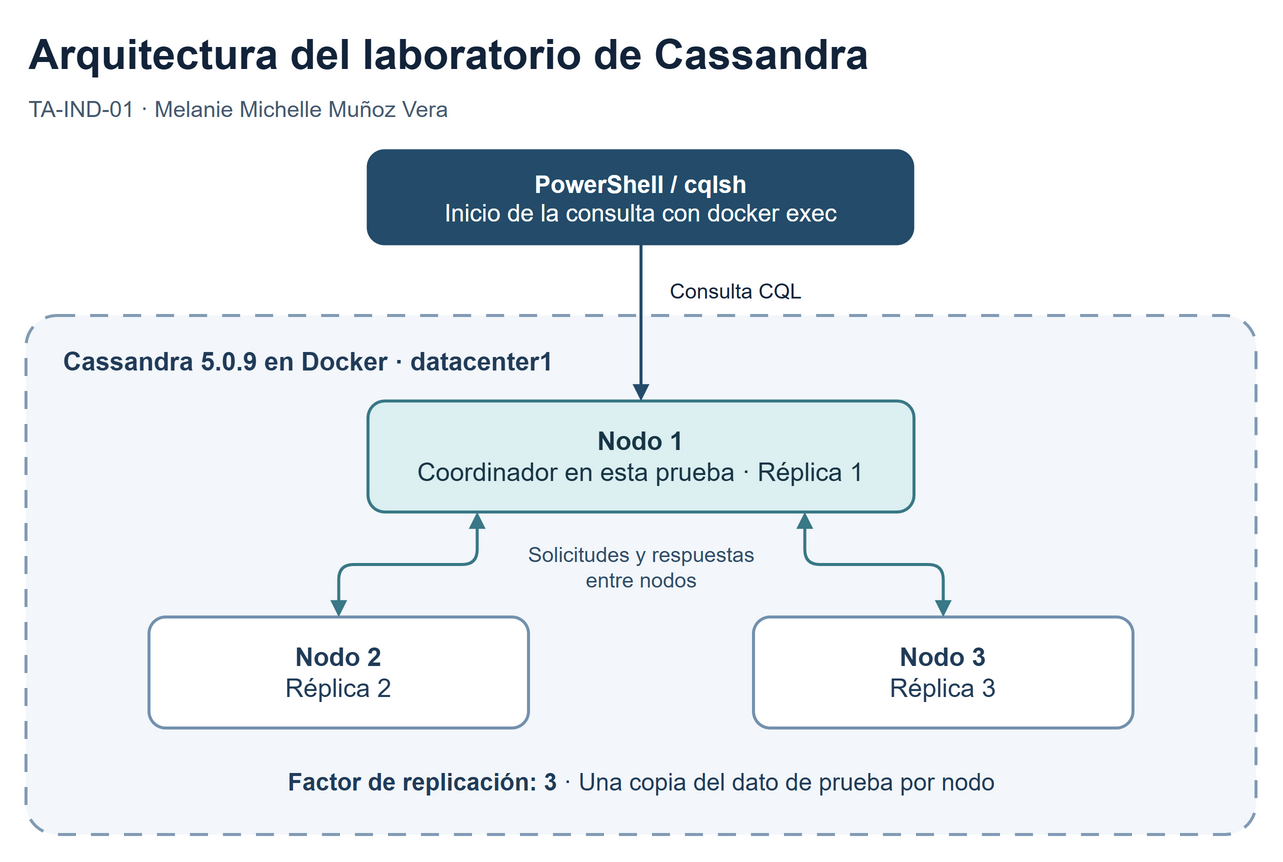
\includegraphics[width=\linewidth,height=0.35\textheight,keepaspectratio]{anexos/cassandra-laboratorio.png}
  \caption{Recorrido de una consulta CQL en el laboratorio. Diagrama elaborado a partir del bosquejo del Anexo~A.}
  \label{fig:cassandra-laboratorio}
\end{figure}

\section{Análisis con los conceptos de la Unidad 1}
\subsection{Transparencias de distribución}
\textbf{Acceso y ubicación.} En la práctica usé la misma consulta CQL para leer la fila con tres nodos y con uno. El coordinador localiza las réplicas mediante la clave de partición. La dirección del nodo al que se conecta el cliente sí forma parte de la configuración \cite{cassandra5dynamo}.

\textbf{Migración y reubicación.} Cassandra puede redistribuir rangos de datos al cambiar la composición del clúster. La consulta conserva la misma clave, pero un cambio de dirección del nodo al que está conectada la sesión puede requerir reconexión. La prueba mantuvo fijo el nodo coordinador y no evaluó movimientos de datos con solicitudes en curso \cite{cassandra5dynamo}.

\textbf{Replicación, concurrencia y fallos.} El coordinador decide qué réplicas contactar según la operación. El cliente sí elige el nivel de consistencia. En escrituras ordinarias que compiten por el mismo dato, Cassandra resuelve el conflicto usando marcas de tiempo \cite{cassandra5dynamo}. En la prueba, la caída fue transparente para la lectura con \texttt{ONE}, que conservó el mismo resultado. Con \texttt{QUORUM}, el error hizo visible la falta de réplicas.
\subsection{CAP y PACELC}
\paragraph{CAP.} Si una partición de red impide que los nodos se comuniquen, el teorema CAP establece que el sistema no puede garantizar a la vez la consistencia linealizable y una respuesta exitosa a toda solicitud que llegue a un nodo operativo \cite{gilbert2002cap}. La prueba de Cassandra permite examinar una consecuencia relacionada. Se detuvieron dos contenedores, de modo que el coordinador solo tenía una réplica disponible. Esa réplica devolvió la fila con \texttt{ONE}. Con \texttt{QUORUM}, el servidor devolvió \texttt{Unavailable} porque necesitaba dos réplicas y solo tenía una activa. El resultado muestra cómo el mínimo de respuestas afecta la disponibilidad de una lectura.

Cassandra permite elegir el nivel de consistencia por operación \cite{cassandra5dynamo}. Con \texttt{ONE}, en otra ejecución, una lectura podría obtener un valor desactualizado si la réplica consultada aún no recibió una escritura reciente. En esta prueba, la fila se insertó con \texttt{ALL} antes de detener los nodos y se leyó sin modificarla. La pérdida de acceso a dos réplicas sirve para ilustrar el dilema de CAP. Comprobar el comportamiento ante una partición real requeriría mantener los nodos activos y bloquear la comunicación entre ellos. Evaluar la consistencia linealizable requeriría además observar el orden de lecturas y escrituras.

\paragraph{PACELC.} El modelo de Abadi plantea una elección entre disponibilidad y consistencia durante una partición (\textit{PAC}), y entre latencia y consistencia cuando la red funciona con normalidad (\textit{ELC}) \cite{abadi2012pacelc}. Con los tres nodos activos, ambas lecturas devolvieron la fila. \texttt{QUORUM} debía esperar dos respuestas para completar la consulta, mientras que a \texttt{ONE} le bastaba una. Esto permite plantear que esperar una segunda respuesta puede aumentar la latencia, sobre todo si una réplica tarda en responder. Las capturas registran el éxito o fallo de la consulta y la hora de cada etapa. Medir la latencia requeriría cronometrar consultas repetidas bajo las mismas condiciones.

Como contraste, Redžepagić et al. midieron la latencia de \emph{escritura} de Cassandra en Kubernetes. En la Tabla~22 de su estudio, el promedio pasó de \(1{,}23\) ms con \texttt{ONE} a \(3{,}16\) ms con \texttt{QUORUM} \cite{redzepagic2026kubernetes}. Esas cifras corresponden a la carga y al entorno de ese estudio. En el laboratorio de este informe, la comparación se limitó a la disponibilidad de una lectura.
\subsection{Modelos de comunicación}
El sistema combina un modelo cliente-servidor entre \texttt{cqlsh} y Cassandra con un modelo entre pares dentro del clúster. El cliente envía solicitudes CQL mediante el protocolo binario nativo sobre TCP y recibe un resultado o un error \cite{cassandra5protocol}. En el laboratorio, cada consulta de la terminal esperó su respuesta. Entre nodos, el coordinador intercambia mensajes con las réplicas y la operación espera las respuestas que exige su nivel de consistencia. El intercambio periódico de estado por \emph{gossip} ocurre en segundo plano \cite{cassandra5dynamo}.
\subsection{Tolerancia a fallos}
La replicación permitió leer la fila aun con dos nodos detenidos. \texttt{nodetool status} mostró dos nodos en \texttt{DN} (caídos, en estado normal dentro del anillo) y uno en \texttt{UN} (activo, en estado normal). Con factor de replicación tres, el umbral de \texttt{ONE} permite tolerar la pérdida de hasta dos réplicas para leer un dato presente en la réplica accesible. \texttt{QUORUM} requiere dos réplicas accesibles y, por tanto, admite la pérdida de una \cite{cassandra5dynamo}. La prueba observó los extremos de tres y una réplica activa.

Tras reiniciar los contenedores, los tres nodos volvieron a \texttt{UN} y la consulta con \texttt{QUORUM} volvió a devolver la fila. Se recuperó así la capacidad de completar esa lectura con el umbral solicitado. Para comprobar la sincronización de las réplicas durante la recuperación, haría falta escribir un dato mientras los otros nodos están detenidos y revisar si lo reciben al volver. Además, los tres contenedores comparten una computadora. Si esta se apaga, los tres nodos quedan fuera de servicio al mismo tiempo.

\paragraph{Incidente en producción.} El equipo de Discord documentó que algunas particiones de mensajes concentraban tantas lecturas que subía la latencia de los nodos responsables. El efecto alcanzaba otras consultas porque las operaciones con cuórum dependían de respuestas de esas réplicas \cite[sección \enquote{Our Cassandra Troubles}]{ingram2023discord}. El caso muestra que una réplica activa también puede degradar el servicio si se satura.

\section{Experimentación propia}
\label{sec:experimento-cassandra}
El 12 de noviembre de 2026 se probó si Cassandra 5.0.9 podía leer una fila escrita previamente, antes, durante y después de detener dos de sus tres nodos. El clúster se ejecutó en Docker, con factor de replicación 3 en \texttt{datacenter1}. Las horas de las capturas corresponden a Ecuador continental (UTC\(\,-5\)). La carpeta \texttt{experimento/} contiene la configuración (\texttt{compose.yaml}, \texttt{preparar.cql}), la secuencia completa (\texttt{COMANDOS.md}) y las salidas registradas (\texttt{RESULTADOS.md}).

\subsection{Preparación del clúster}
Desde la carpeta \texttt{experimento}, el clúster se levantó en PowerShell y se cargó el esquema de la tabla \texttt{ta\_ind\_01.prueba}. El primer \texttt{nodetool status} mostró los tres nodos activos (Figura~\ref{fig:exp-nodos}).

{\small
\begin{verbatim}
$docker = "$env:LOCALAPPDATA\Programs\DockerDesktop\resources\bin\docker.exe"
$nodo = 'ta-ind-cassandra-nodo1-1'
& $docker compose -f compose.yaml up -d --wait --wait-timeout 420
& $docker exec $nodo nodetool status
Get-Content -Raw preparar.cql | & $docker exec -i $nodo cqlsh
\end{verbatim}
}

\begin{figure}[H]
  \centering
  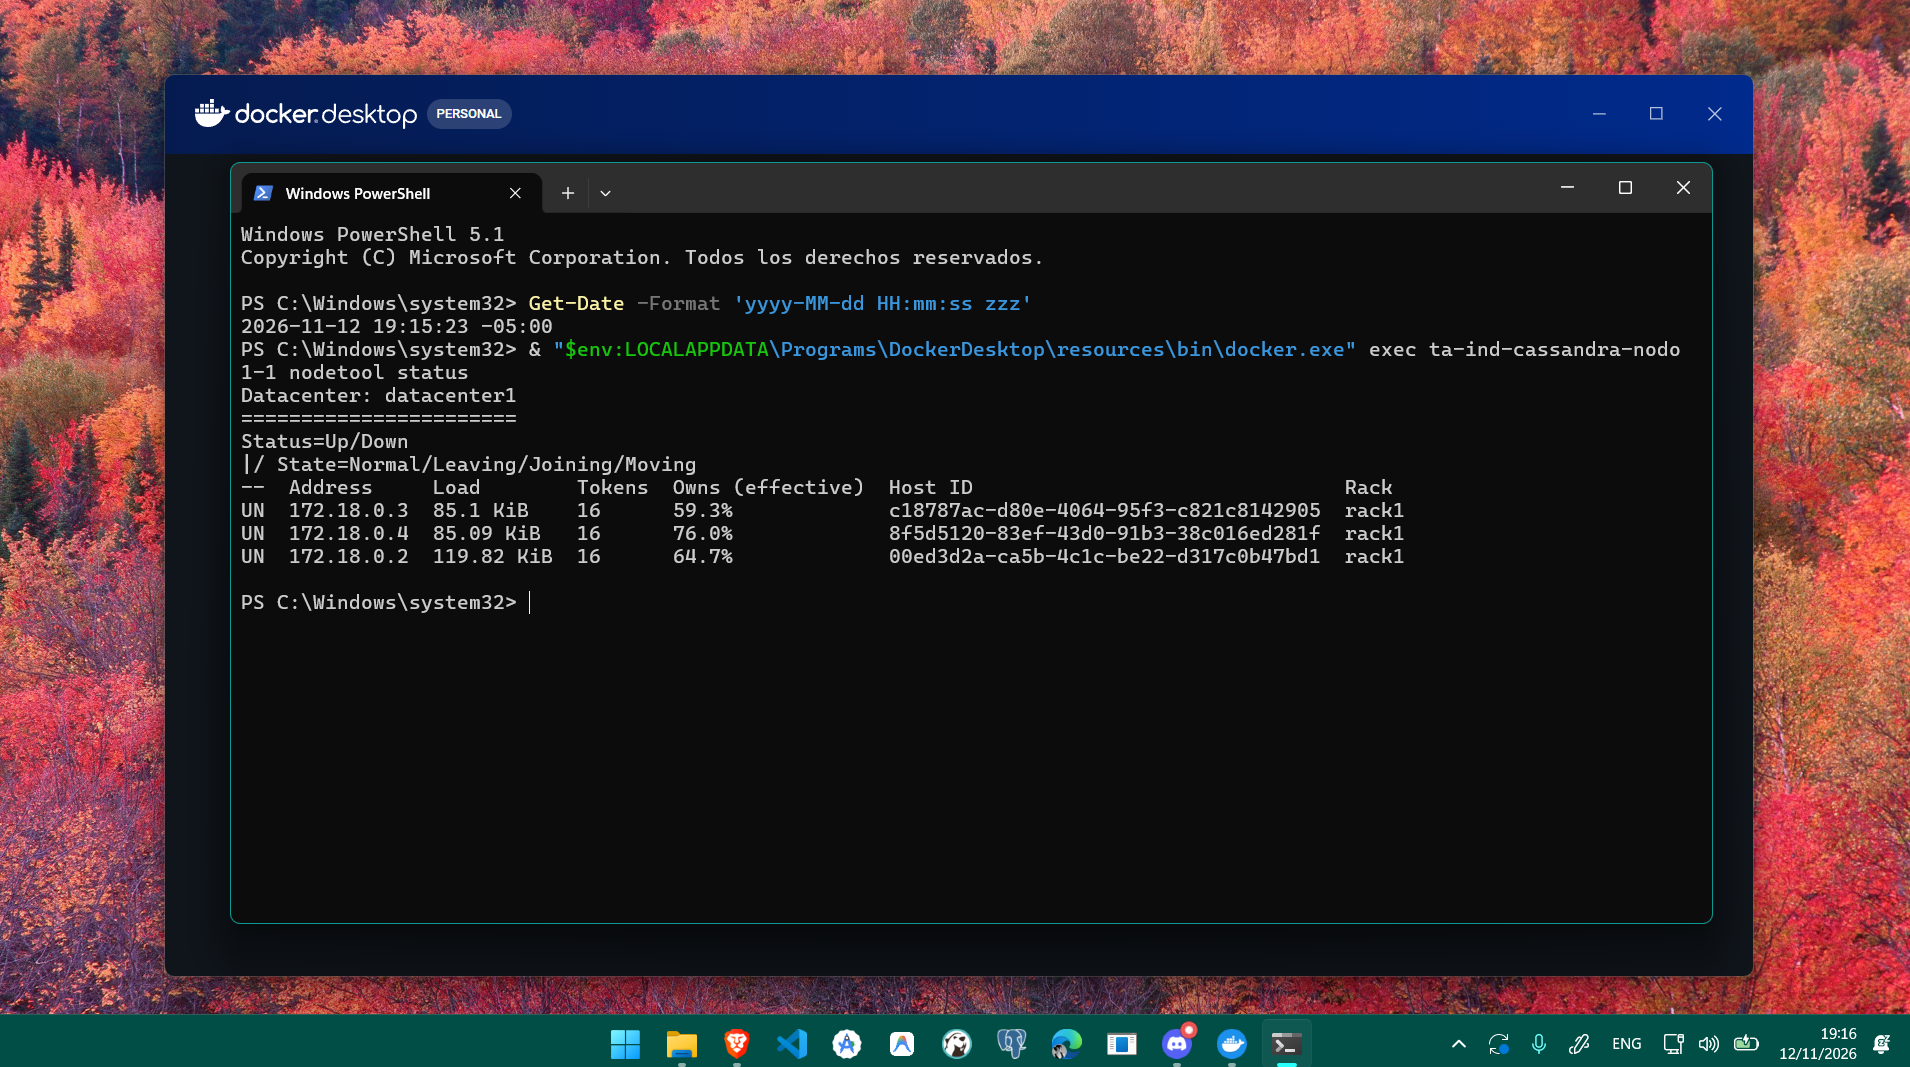
\includegraphics[width=\linewidth,height=.24\textheight,keepaspectratio]{experimento/capturas/01-tres-nodos-activos.png}
  \caption{Estado inicial a las 19:15:23. Los tres nodos aparecen como \texttt{UN}.}
  \label{fig:exp-nodos}
\end{figure}

\subsection{Antes de la caída}
La fila se insertó con \texttt{ALL}. Luego se consultó el mismo identificador con \texttt{ONE} y \texttt{QUORUM}. Ambas lecturas devolvieron la fila 1 con el mensaje \enquote{Prueba de Melanie} (Figura~\ref{fig:exp-antes}).

{\small
\begin{verbatim}
Get-Date -Format 'yyyy-MM-dd HH:mm:ss zzz'
@'
CONSISTENCY ALL;
INSERT INTO ta_ind_01.prueba (id, mensaje) VALUES (1, 'Prueba de Melanie');
CONSISTENCY ONE;
SELECT * FROM ta_ind_01.prueba WHERE id = 1;
CONSISTENCY QUORUM;
SELECT * FROM ta_ind_01.prueba WHERE id = 1;
'@ | & $docker exec -i $nodo cqlsh
\end{verbatim}
}

\begin{figure}[H]
  \centering
  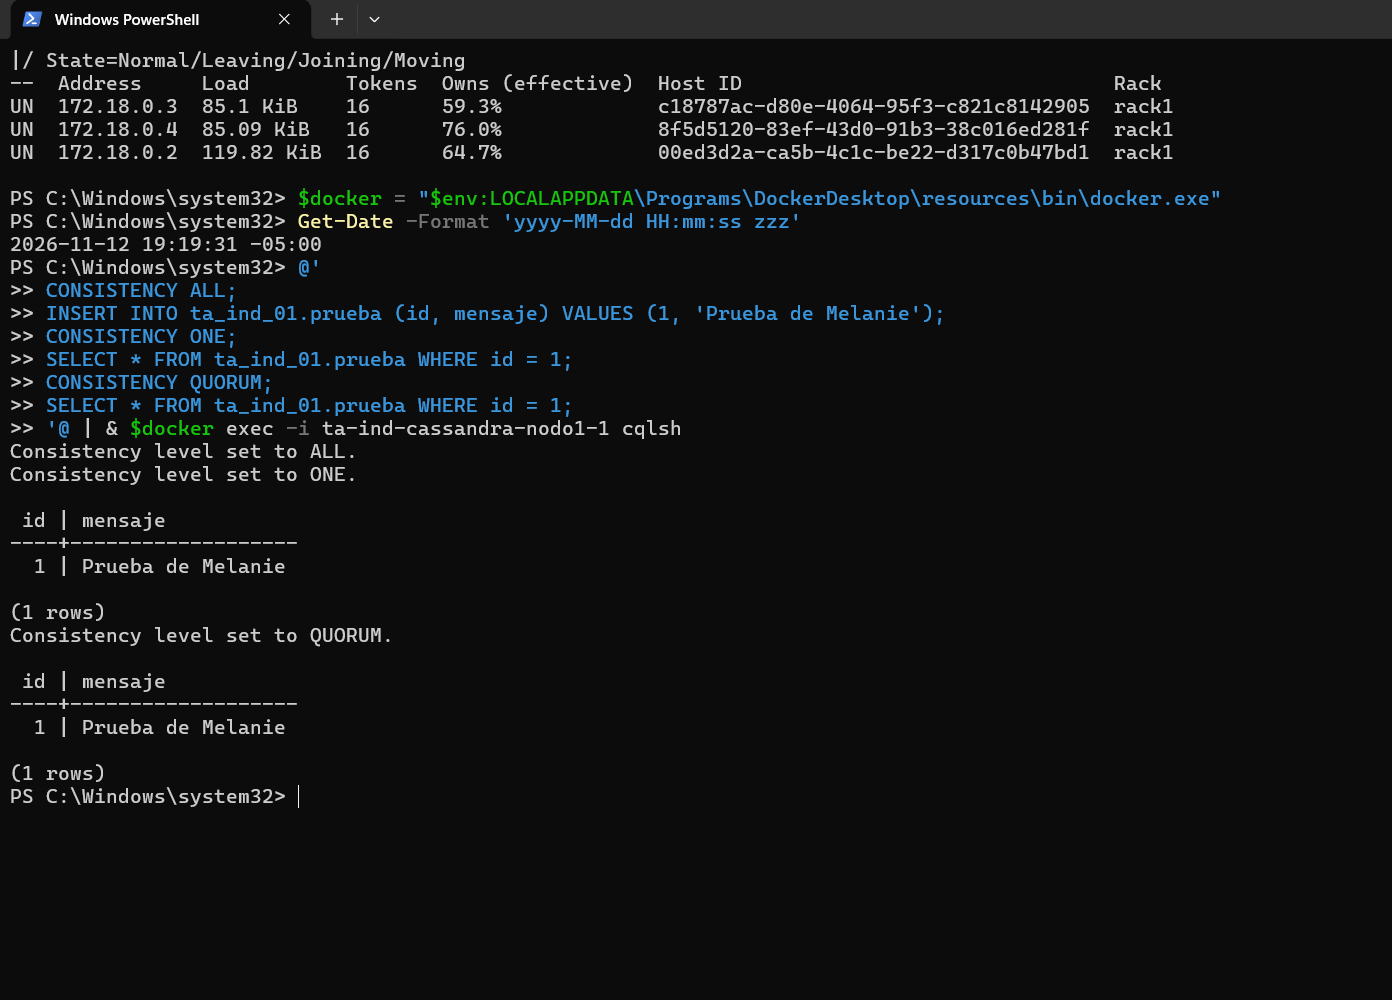
\includegraphics[width=\linewidth,height=.32\textheight,keepaspectratio]{experimento/capturas/02-lecturas-con-tres-nodos.png}
  \caption{Escritura con \texttt{ALL} y lecturas con tres nodos activos a las 19:19:31.}
  \label{fig:exp-antes}
\end{figure}

\subsection{Durante la caída}
Se detuvieron los contenedores \texttt{nodo2} y \texttt{nodo3}. Cuando \texttt{nodetool status} mostró una fila \texttt{UN} y dos \texttt{DN}, se repitieron las lecturas desde el nodo 1.

{\small
\begin{verbatim}
& $docker compose -f compose.yaml stop nodo2 nodo3
Get-Date -Format 'yyyy-MM-dd HH:mm:ss zzz'
& $docker exec $nodo nodetool status
@'
CONSISTENCY ONE;
SELECT * FROM ta_ind_01.prueba WHERE id = 1;
CONSISTENCY QUORUM;
SELECT * FROM ta_ind_01.prueba WHERE id = 1;
'@ | & $docker exec -i $nodo cqlsh
\end{verbatim}
}

\texttt{ONE} devolvió la fila 1. Con \texttt{QUORUM}, el servidor devolvió \texttt{Unavailable}. El cliente \texttt{cqlsh} mostró \texttt{NoHostAvailable}. El detalle del error indicó \texttt{required\_replicas = 2} y \texttt{alive\_replicas = 1} (Figura~\ref{fig:exp-durante}).

\begin{figure}[H]
  \centering
  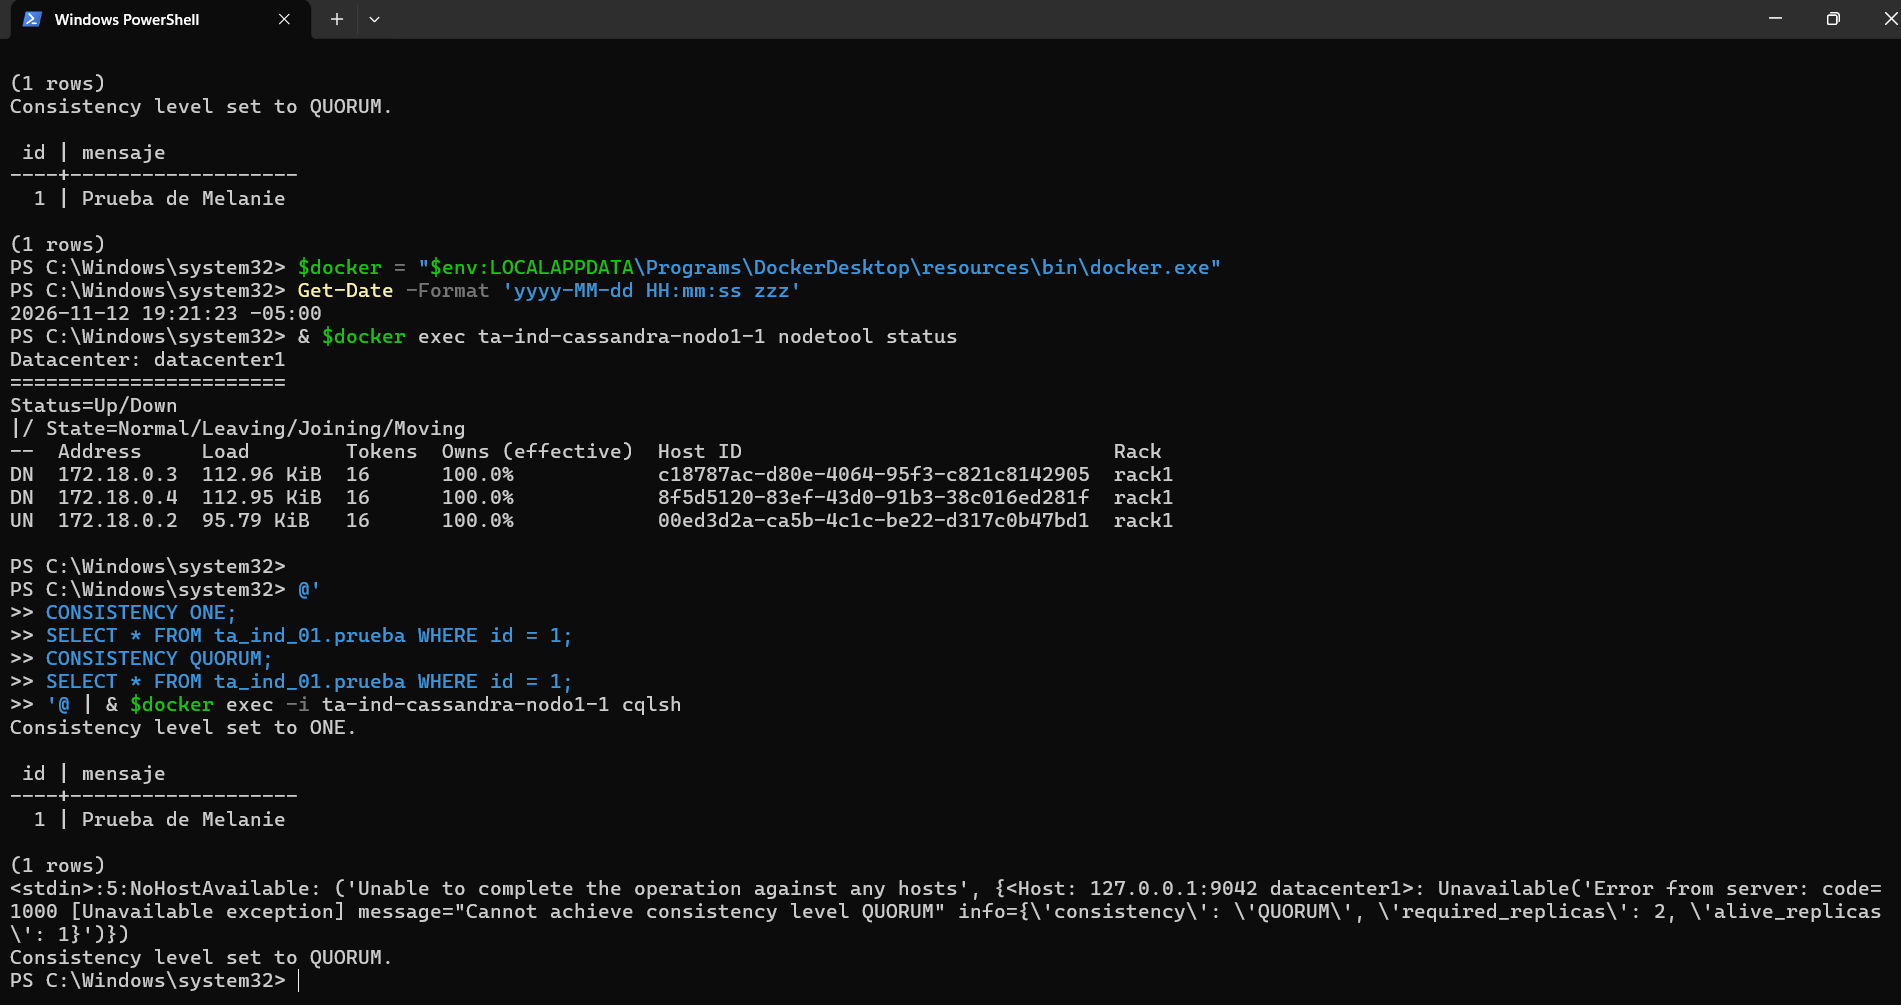
\includegraphics[width=\linewidth]{experimento/capturas/03-lecturas-con-un-nodo.png}
  \caption{Lecturas con un nodo activo a las 19:21:23. El error de \texttt{QUORUM} aparece al final de la captura.}
  \label{fig:exp-durante}
\end{figure}

\subsection{Después de la recuperación}
Se levantaron de nuevo los contenedores detenidos y se repitió la lectura con \texttt{QUORUM}. Los tres nodos volvieron a aparecer como \texttt{UN} y la consulta devolvió la fila 1 (Figura~\ref{fig:exp-despues}).

{\small
\begin{verbatim}
& $docker compose -f compose.yaml up -d --wait --wait-timeout 360
Get-Date -Format 'yyyy-MM-dd HH:mm:ss zzz'
& $docker exec $nodo nodetool status
$consulta = 'CONSISTENCY QUORUM; SELECT * FROM ta_ind_01.prueba WHERE id = 1;'
& $docker exec $nodo cqlsh -e $consulta
\end{verbatim}
}

\begin{figure}[H]
  \centering
  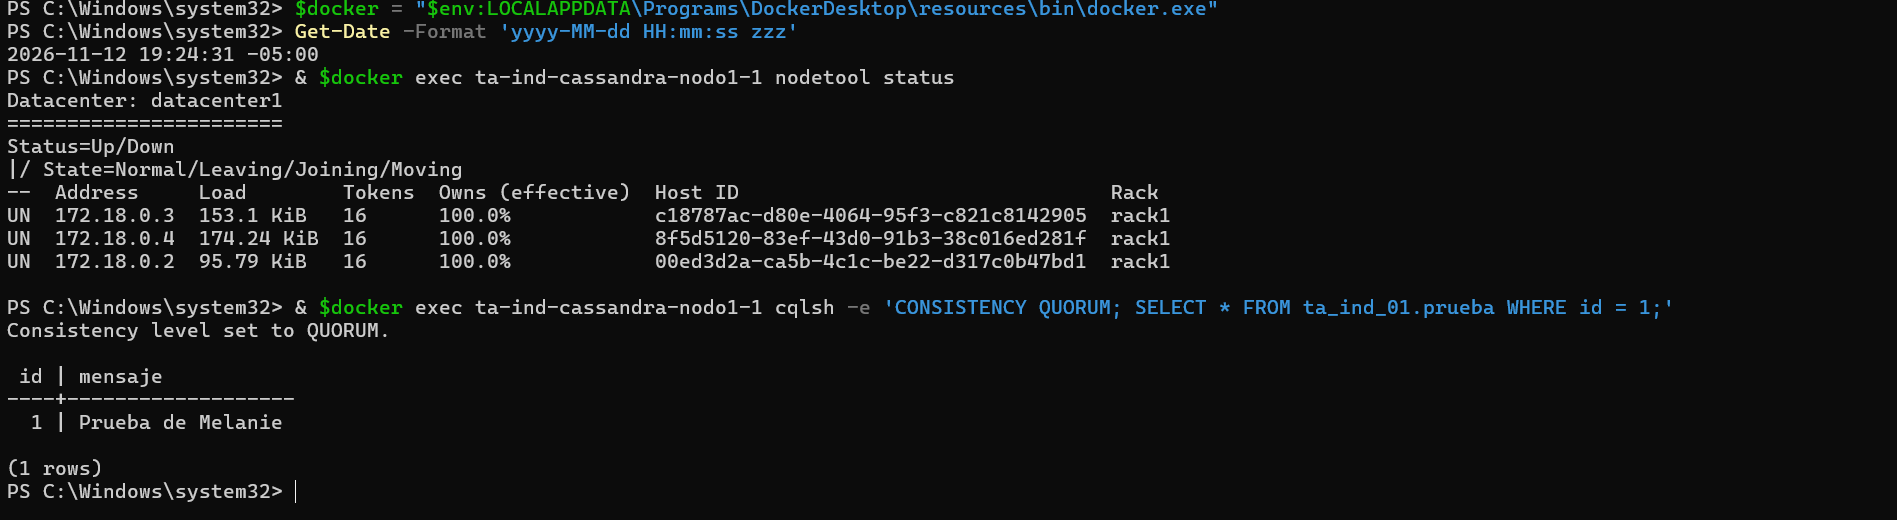
\includegraphics[width=\linewidth]{experimento/capturas/04-lectura-quorum-recuperada.png}
  \caption{Lectura con \texttt{QUORUM} tras la recuperación a las 19:24:31.}
  \label{fig:exp-despues}
\end{figure}

\begin{table}[H]
  \centering
  \caption{Resultados de las lecturas de la fila 1 por etapa.}
  \label{tab:exp-cassandra}
  \begin{tabular}{@{}lcll@{}}
    \toprule
    Etapa & Nodos activos & \texttt{ONE} & \texttt{QUORUM} \\
    \midrule
    Antes de la caída & 3 & Devuelve la fila & Devuelve la fila \\
    Durante la caída & 1 & Devuelve la fila & \texttt{Unavailable} \\
    Tras la recuperación & 3 & Sin nueva consulta & Devuelve la fila \\
    \bottomrule
  \end{tabular}
\end{table}

\section{Ejemplos de mi entorno}

\subsection{Comunicación del tema por WhatsApp}
Para esta actividad comuniqué mi tema en el grupo de WhatsApp de la asignatura. Envié un mensaje indicando que analizaría Apache Cassandra y lo compararía con MongoDB. En la conversación, mi mensaje aparece a las 17:46 y después se ven los temas que anunciaron otros compañeros a las 17:47 y 17:49.

Esta interacción ilustra la comunicación asíncrona entre personas. Cada integrante puede enviar su propuesta y los demás pueden consultarla y responder en otro momento. Las horas visibles permiten seguir el orden de los mensajes mostrados en mi pantalla. También se aprecia la transparencia de ubicación desde la perspectiva de uso. Para comunicar mi elección seleccioné el grupo, sin tener que conocer la ubicación física de los dispositivos de mis compañeros ni de los servidores del servicio.

\subsection{Consulta de versiones del informe en GitHub}
Al revisar el repositorio de esta actividad en GitHub, pude ver que el PDF del análisis de la Unidad~1 y el PDF de la experimentación quedaron en dos commits distintos, \texttt{4da2559} y \texttt{e601a2a}. El historial me permite identificar en qué versión se agregó cada PDF y consultar la versión del archivo que corresponde a ese commit.

Este ejemplo también muestra cómo se comunican dos partes de un sistema distribuido. Git permite trabajar sobre una copia local del repositorio y publicar cambios en el repositorio remoto \cite{githubCloningRepo}. Al consultar GitHub desde el navegador, se ve el estado publicado. Que una edición local todavía no aparezca en la web es una consecuencia de ese paso explícito de publicación. En la prueba de Cassandra, en cambio, el coordinador se comunica con las réplicas para atender la lectura en curso según el nivel solicitado. En ambos casos es necesario distinguir qué copias intervienen para interpretar lo que se ve en pantalla.

\section{Análisis comparativo}
La Tabla~\ref{tab:cassandra-mongodb} compara Cassandra 5.0 con MongoDB 8.0 en un conjunto de réplicas. MongoDB 8.0 se publicó en octubre de 2024 \cite{mongodb2024release}. Ambos mantienen copias de los datos en varios nodos. La prueba de la Sección~\ref{sec:experimento-cassandra} aporta evidencia para Cassandra. Los escenarios de MongoDB se analizan a partir de su documentación.

\begin{table}[H]
  \centering
  \caption{Cassandra y MongoDB según seis criterios de la Unidad 1.}
  \label{tab:cassandra-mongodb}
  \small
  \renewcommand{\arraystretch}{1.14}
  \begin{tabularx}{\linewidth}{@{}p{.20\linewidth}XX@{}}
    \toprule
    \textbf{Criterio} & \textbf{Cassandra 5.0} & \textbf{MongoDB 8.0} \\
    \midrule
    Modelo de comunicación &
    Un nodo coordina la solicitud del cliente. Los nodos intercambian información de estado mediante \emph{gossip} \cite{cassandra5dynamo}. &
    El primario recibe las escrituras del cliente. Los secundarios replican las operaciones de forma asíncrona \cite{mongodb8replication}. \\
    \addlinespace
    Transparencia de replicación &
    El coordinador localiza las réplicas de la partición. El cliente puede elegir el nivel de consistencia \cite{cassandra5dynamo}. &
    El conjunto mantiene copias de los datos. El cliente puede configurar qué miembros usar para las lecturas \cite{mongodb8replication}. \\
    \addlinespace
    Consistencia de lectura &
    Con tres réplicas, \texttt{ONE} pide una respuesta y \texttt{QUORUM} pide dos \cite{cassandra5dynamo}. &
    Una lectura \texttt{linearizable} en el primario puede reflejar, para un documento, todas las escrituras previas confirmadas por mayoría \cite{mongodb8linearizable}. \\
    \addlinespace
    Partición de red (CAP) &
    Con acceso a una sola de tres réplicas, el coordinador puede leer con \texttt{ONE}. Con \texttt{QUORUM} necesita dos accesibles \cite{cassandra5dynamo}. &
    El primario del lado minoritario pierde su rol al detectar que dejó de comunicarse con la mayoría de votantes \cite{mongodb8elections}. \\
    \addlinespace
    Latencia (PACELC) &
    En operación normal, esperar dos respuestas con \texttt{QUORUM} puede alargar una lectura frente a \texttt{ONE} \cite{cassandra5dynamo,abadi2012pacelc}. &
    Una lectura \texttt{linearizable} puede esperar a que las escrituras concurrentes se propaguen a la mayoría \cite{mongodb8linearizable}. \\
    \addlinespace
    Tolerancia y recuperación &
    Con tres réplicas, las lecturas con \texttt{QUORUM} pueden continuar si dos son accesibles. Otro nodo puede coordinar una nueva solicitud \cite{cassandra5dynamo}. &
    Si el primario falla, la mayoría de los votantes permite elegir un nuevo primario elegible. Durante la elección se interrumpen las escrituras \cite{mongodb8elections}. \\
    \bottomrule
  \end{tabularx}
\end{table}

\subsection{Discusión}
En el laboratorio, la fila ya estaba escrita con \texttt{ALL} cuando detuve dos contenedores. Con una réplica activa, \texttt{ONE} devolvió la fila y \texttt{QUORUM} produjo el error \texttt{Unavailable}. En Cassandra se cuentan respuestas de las réplicas de la partición para esa operación. En MongoDB se cuentan votos del conjunto para mantener o elegir un primario. Si solo queda accesible uno de tres votantes, el conjunto pierde el primario al detectar la falta de mayoría y se interrumpen las escrituras. Una lectura podría seguir disponible en un secundario si la configuración del cliente y el nivel de lectura lo permiten \cite{mongodb8replication,mongodb8elections}.

La elección depende de lo que la aplicación necesite garantizar. Para una consulta que tolera datos desactualizados, \texttt{ONE} permite aprovechar la réplica accesible. Para una consulta de un documento que deba reflejar todas las escrituras previas confirmadas por mayoría, MongoDB ofrece \texttt{linearizable} bajo las condiciones indicadas en su manual \cite{mongodb8linearizable}. El umbral de lectura \texttt{QUORUM} por sí solo cuenta respuestas. La garantía sobre el dato también depende del nivel de escritura y de las operaciones concurrentes \cite{cassandra5dynamo}.

La prueba local registró si la consulta pudo completarse. Para comparar tiempos habría que controlar la carga, la red y las garantías solicitadas. Ferreira et al. usaron \texttt{ONE} y \texttt{ALL} en Cassandra, y compararon lecturas \texttt{local} y \texttt{linearizable} en MongoDB en su propio entorno \cite[sección \enquote{Database configurations}]{ferreira2024cloud}. Sus mediciones corresponden a esas configuraciones.

\section{Postura crítica}
\paragraph{Fortalezas.} Considero que la principal ventaja de Cassandra es poder ajustar el nivel de consistencia a lo que necesita cada operación. Al detener dos de los tres nodos, la lectura con \texttt{ONE} todavía devolvió la fila que había escrito antes de la caída. Esto resulta útil para consultas en las que importa seguir respondiendo y se puede tolerar que una réplica devuelva un dato desactualizado. La arquitectura también permite que distintos nodos coordinen solicitudes sin elegir un primario para el clúster \cite{cassandra5dynamo}.

\paragraph{Limitaciones.} Con dos nodos detenidos, \texttt{QUORUM} devolvió \texttt{Unavailable} porque quedaba una réplica activa y se necesitaban dos. La consulta volvió a funcionar cuando levanté los nodos. El resultado demuestra que la disponibilidad depende del nivel solicitado. Mi prueba se limita a una fila escrita con \texttt{ALL}, a lecturas sin escrituras concurrentes y a tres contenedores en una sola computadora. Por eso, el resultado sirve para evaluar la pérdida de nodos en esa configuración. Comparar la latencia o evaluar una partición de red exigiría pruebas específicas.

\paragraph{Cuándo elegiría otra opción.} Para una aplicación en la que una decisión dependa del estado más reciente de un documento, como confirmar si un pedido ya fue cancelado, evitaría usar una lectura de Cassandra con \texttt{ONE}. Si el requisito es reflejar todas las escrituras previas confirmadas por mayoría sobre ese documento, consideraría MongoDB con lectura \texttt{linearizable} en el primario y escrituras confirmadas por mayoría \cite{mongodb8linearizable}. Aceptaría que, si un conjunto de tres votantes pierde la mayoría, se interrumpan las escrituras hasta recuperar un primario \cite{mongodb8elections}. En ese caso, me parece preferible que la operación espere o devuelva un error a que la aplicación actúe con un estado desactualizado.

El costo de una configuración también depende de la carga. Nejati Sharif Aldin y Nayebi Pour estudiaron cómo interactúan los niveles de consistencia, la estrategia de replicación y la frecuencia del procesador al evaluar el rendimiento y el consumo energético de Cassandra \cite{nejati2026cassandra}. Mi prueba observó si una lectura podía completarse. Esas otras métricas requerirían mediciones propias.

\section{Conclusiones}
Con factor de replicación tres, una réplica activa bastó para leer con \texttt{ONE} una fila que ya estaba escrita. El mismo nodo devolvió un error con \texttt{QUORUM} porque ese nivel exigía dos respuestas. Al restaurar los tres nodos, la misma lectura con \texttt{QUORUM} volvió a completarse.

La disponibilidad debe analizarse por operación. En Cassandra, el nivel de consistencia determina el mínimo de respuestas para la consulta. En un conjunto de réplicas de MongoDB, la mayoría de votantes permite mantener o elegir al primario que recibe las escrituras \cite{cassandra5dynamo,mongodb8elections}. Para elegir entre ambos, primero definiría qué lecturas y escrituras deben seguir disponibles y cuánto retraso en la actualización de los datos puede aceptar la aplicación. El montaje local permitió observar el efecto de perder nodos. Quedan por evaluar la latencia y el comportamiento bajo una partición de red.

\section*{Declaración de uso de inteligencia artificial}
Usé Gemini 4 Argon de Google para traducir fragmentos de las referencias en inglés. Usé Codex de OpenAI para guiar la configuración y la práctica de Cassandra, localizar fuentes y apoyar la redacción, la corrección del texto y la preparación del archivo LaTeX. Para el análisis se consultaron las publicaciones originales y se cotejaron sus datos bibliográficos. Los resultados de la práctica se contrastaron con los comandos y las salidas visibles en las cuatro capturas originales. La versión exacta de Codex utilizada durante la práctica no quedó registrada.

\clearpage
\printbibliography[title={Referencias}]

\clearpage
\appendix
\section{Esquema inicial a mano}
El bosquejo sirvió de base para el diagrama de la arquitectura. En la versión digital se distingue \texttt{cqlsh} dentro del flujo de PowerShell y se mantiene el papel del nodo 1 como coordinador de la prueba.

\begin{figure}[H]
  \centering
  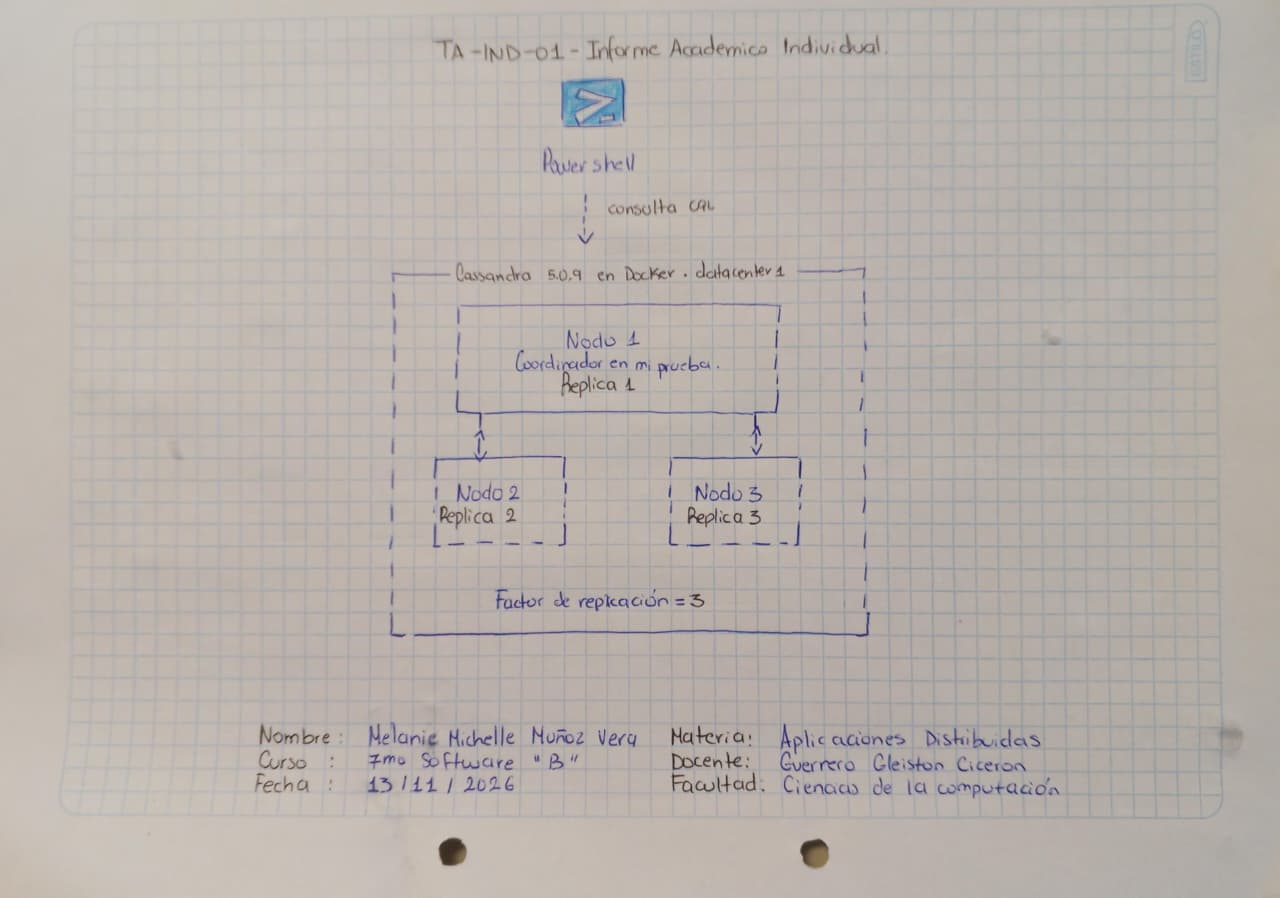
\includegraphics[width=\linewidth]{anexos/bosquejo-cassandra-original.png}
  \caption{Fotografía del bosquejo original del clúster de Cassandra.}
\end{figure}

\clearpage
\section{Lectura de las fuentes}
\begin{figure}[H]
  \centering
  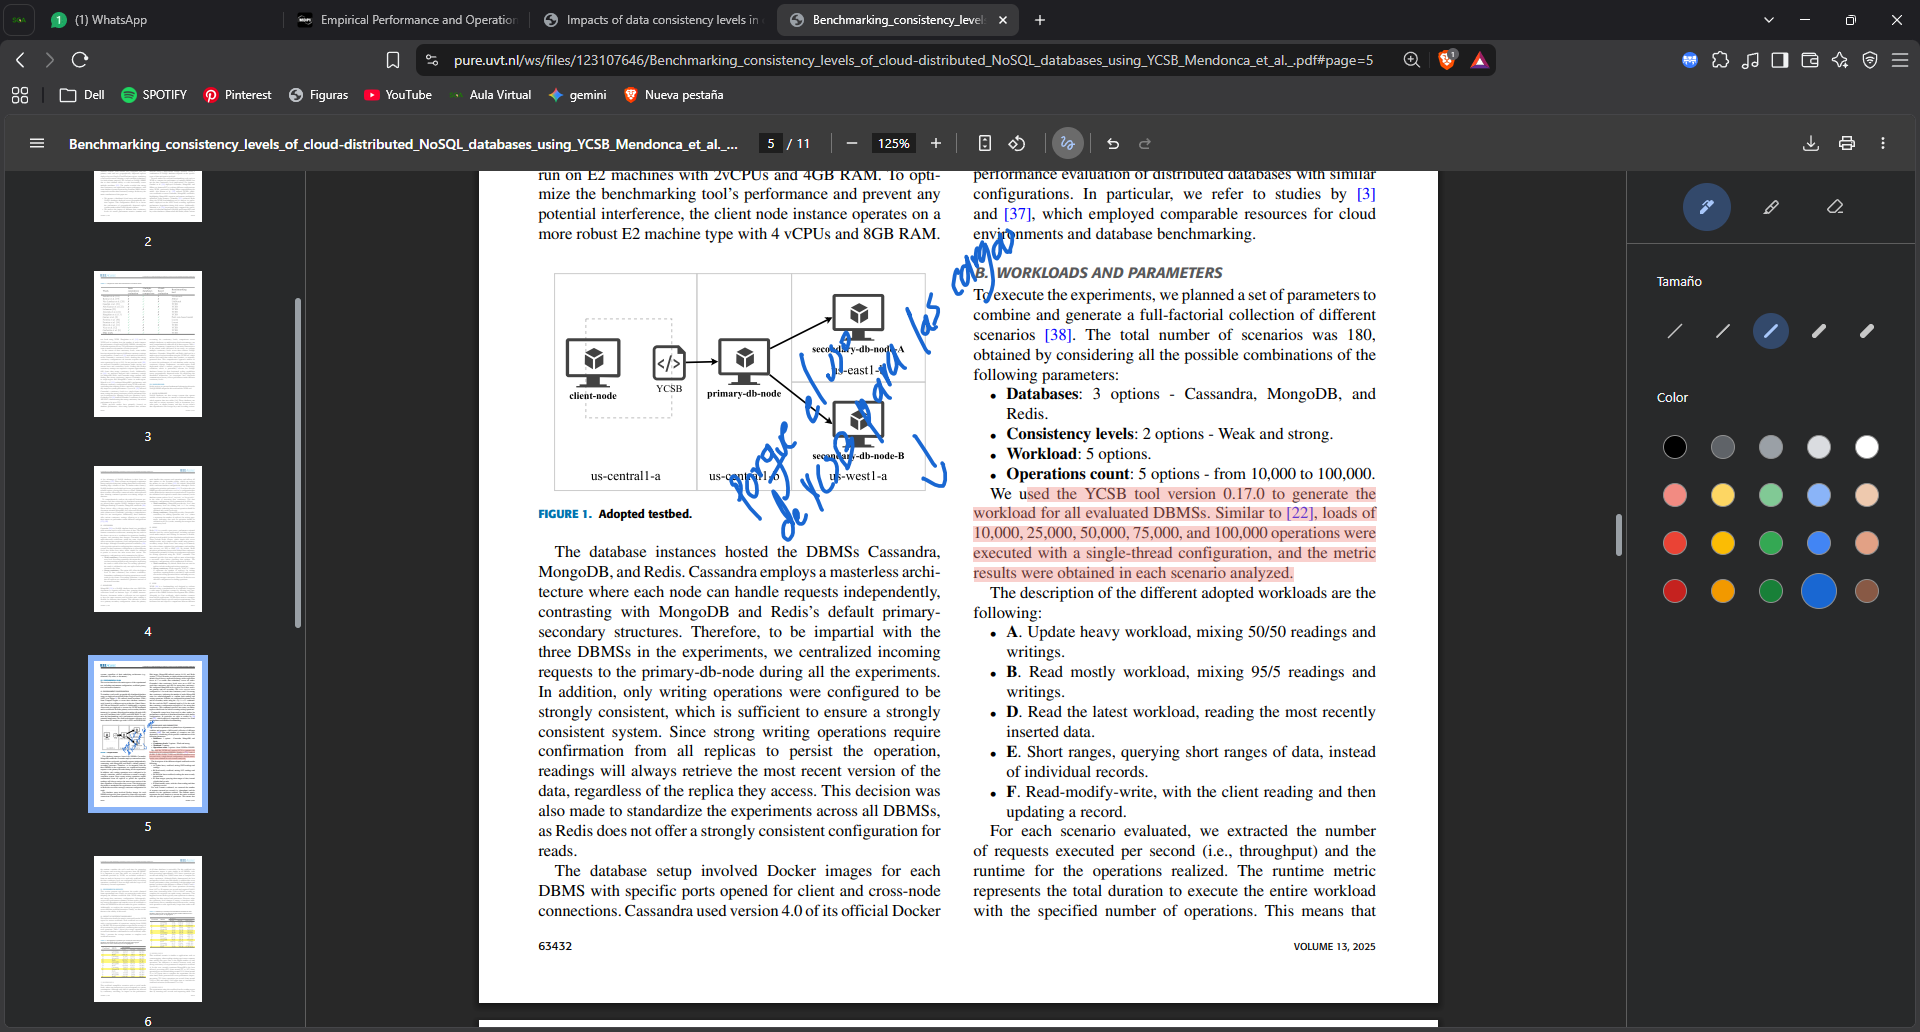
\includegraphics[width=\linewidth,height=.36\textheight,keepaspectratio]{anexos/lectura/ieee-access-2025-p63432.png}
  \caption{Ferreira et al., p.~63432. Sección sobre las cargas y los parámetros de YCSB \cite{ferreira2025ycsb}.}
\end{figure}

\begin{figure}[H]
  \centering
  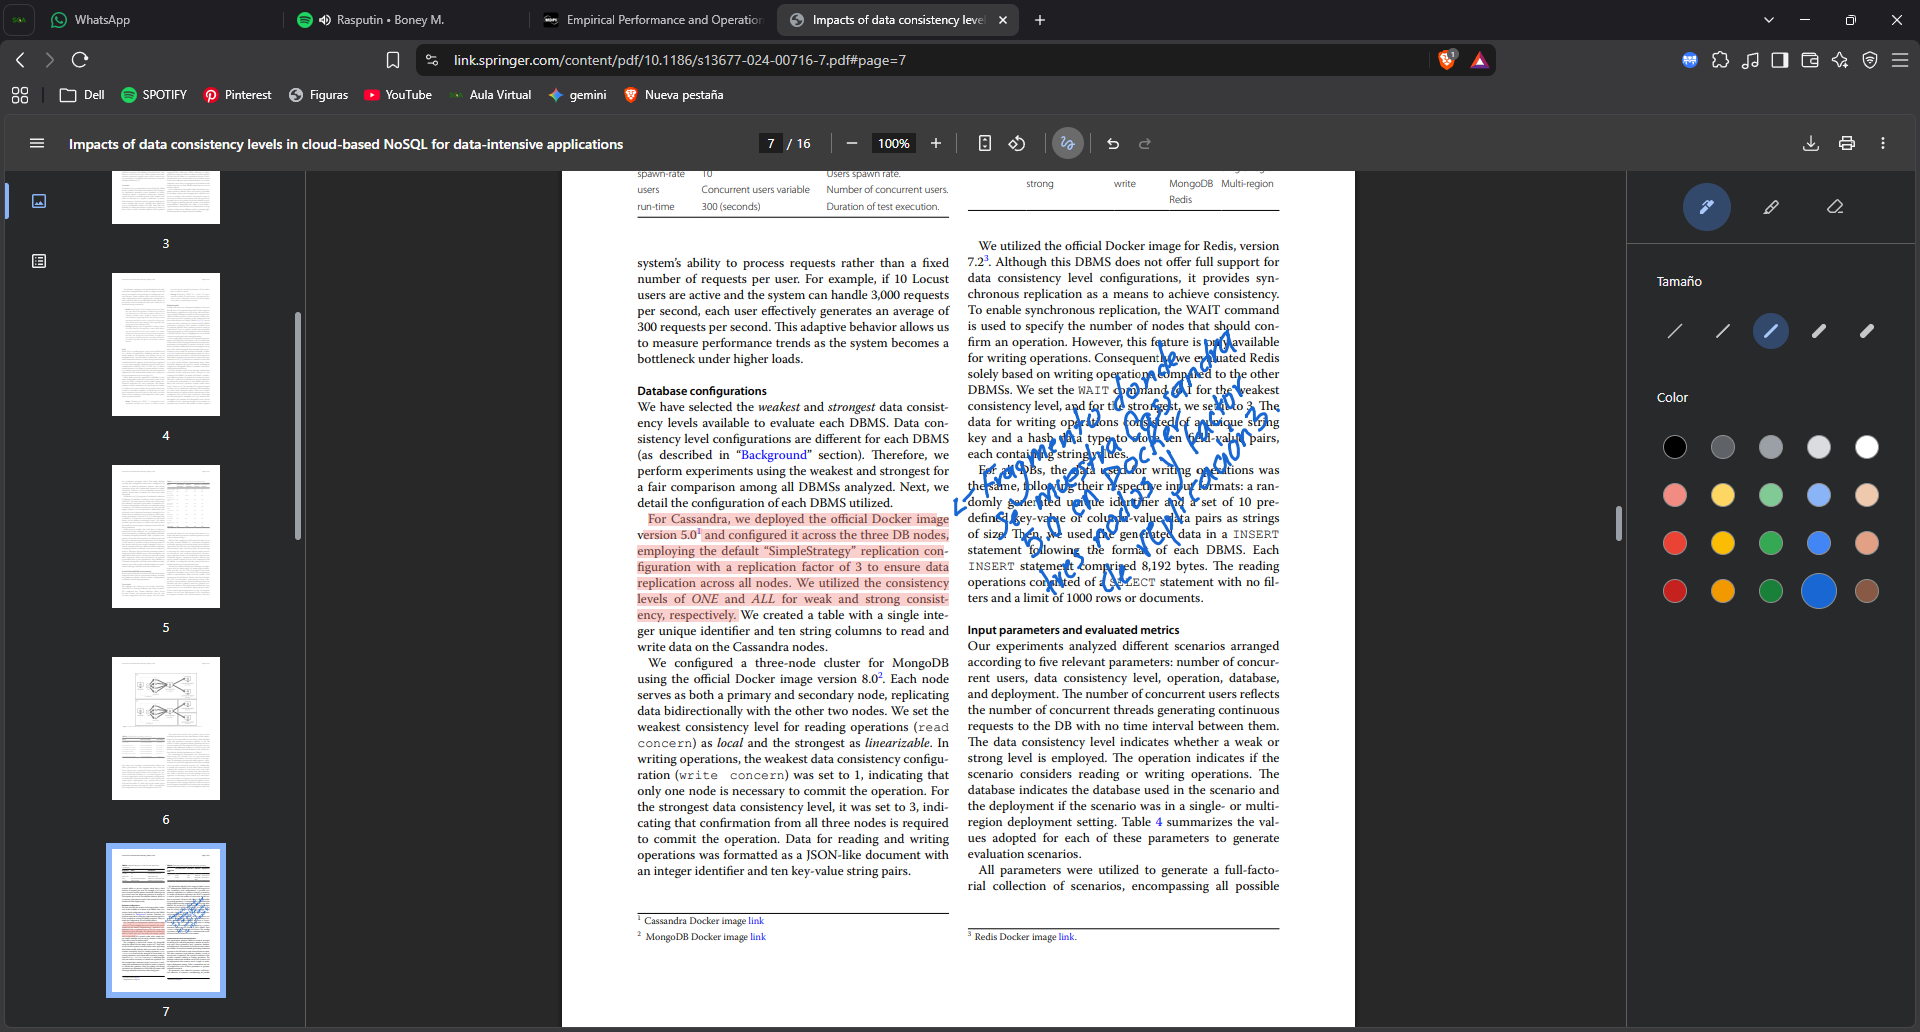
\includegraphics[width=\linewidth,height=.36\textheight,keepaspectratio]{anexos/lectura/journal-cloud-computing-2024-p07.png}
  \caption{Ferreira et al., p.~7 del PDF. Configuración de Cassandra con tres nodos y niveles \texttt{ONE} y \texttt{ALL} \cite{ferreira2024cloud}.}
\end{figure}

\begin{figure}[H]
  \centering
  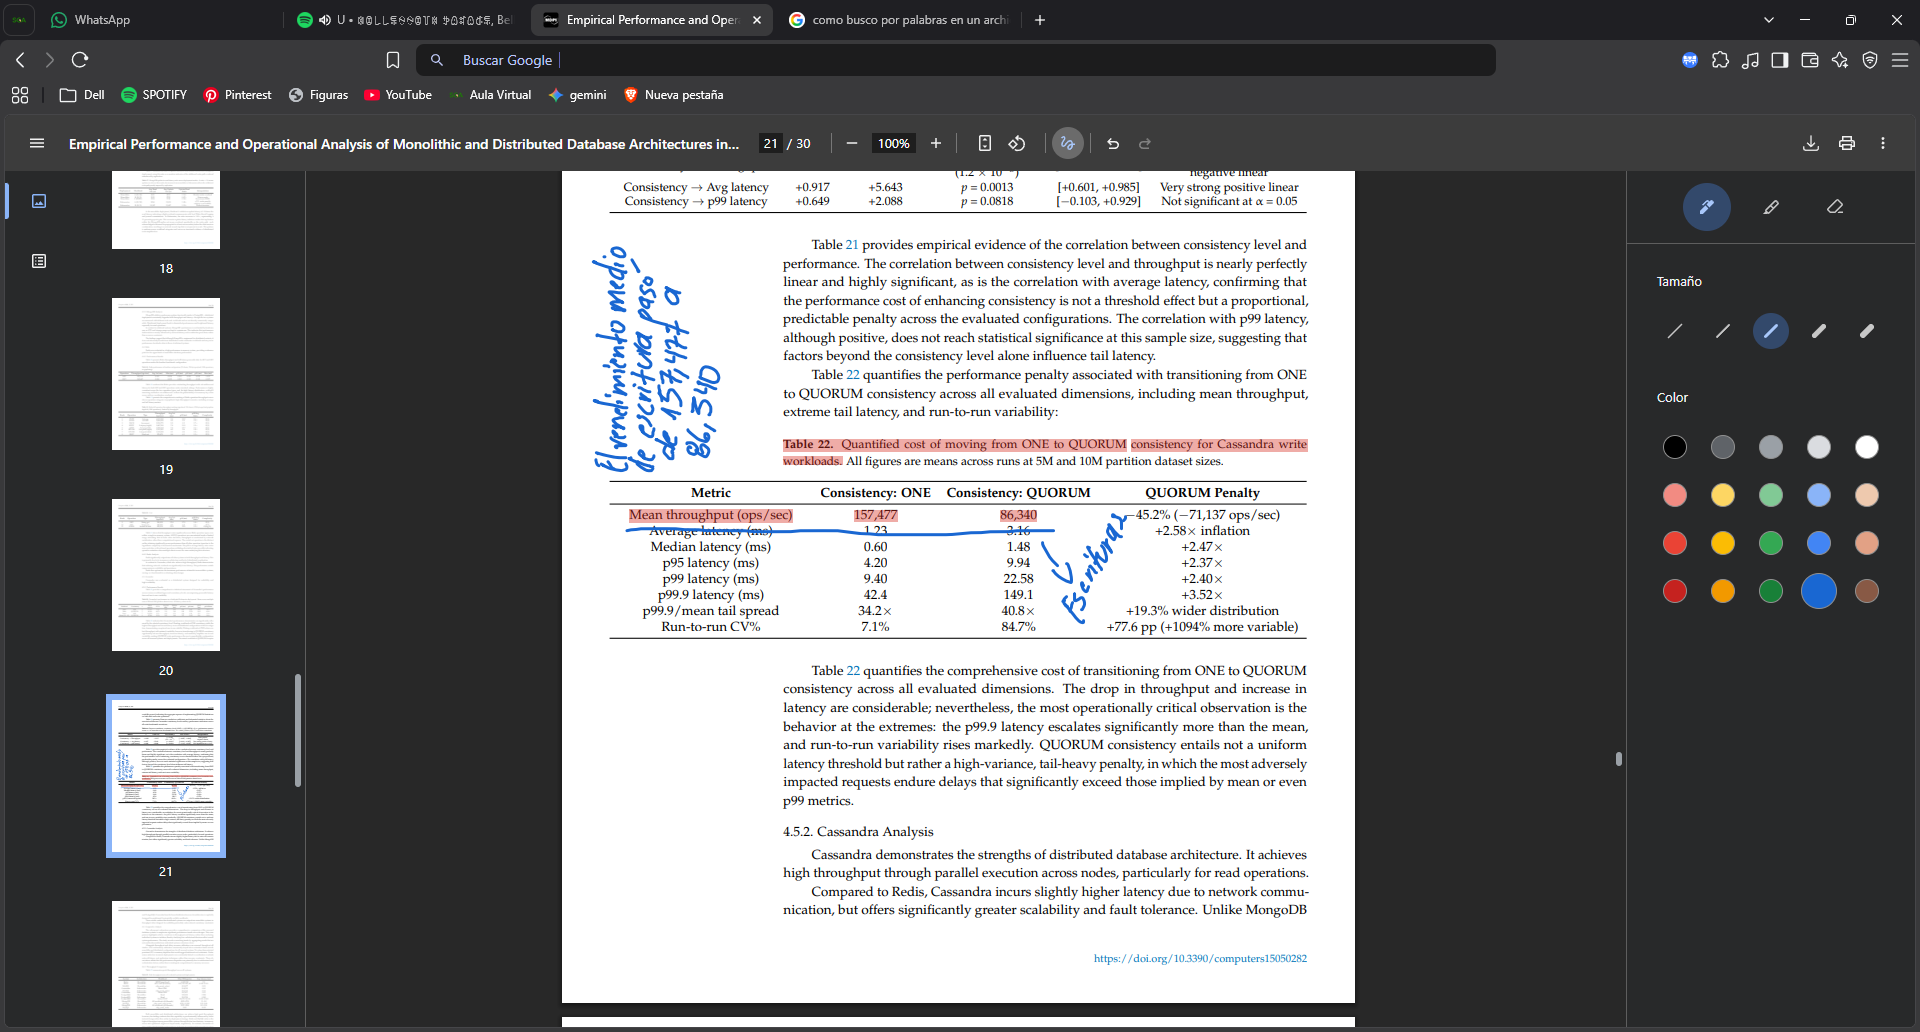
\includegraphics[width=\linewidth]{anexos/lectura/computers-2026-p21.png}
  \caption{Redžepagić et al., p.~21 del PDF. Tabla 22 sobre el rendimiento de escritura con \texttt{ONE} y \texttt{QUORUM} \cite{redzepagic2026kubernetes}.}
\end{figure}
\end{document}
